\subsection{Property View Models}


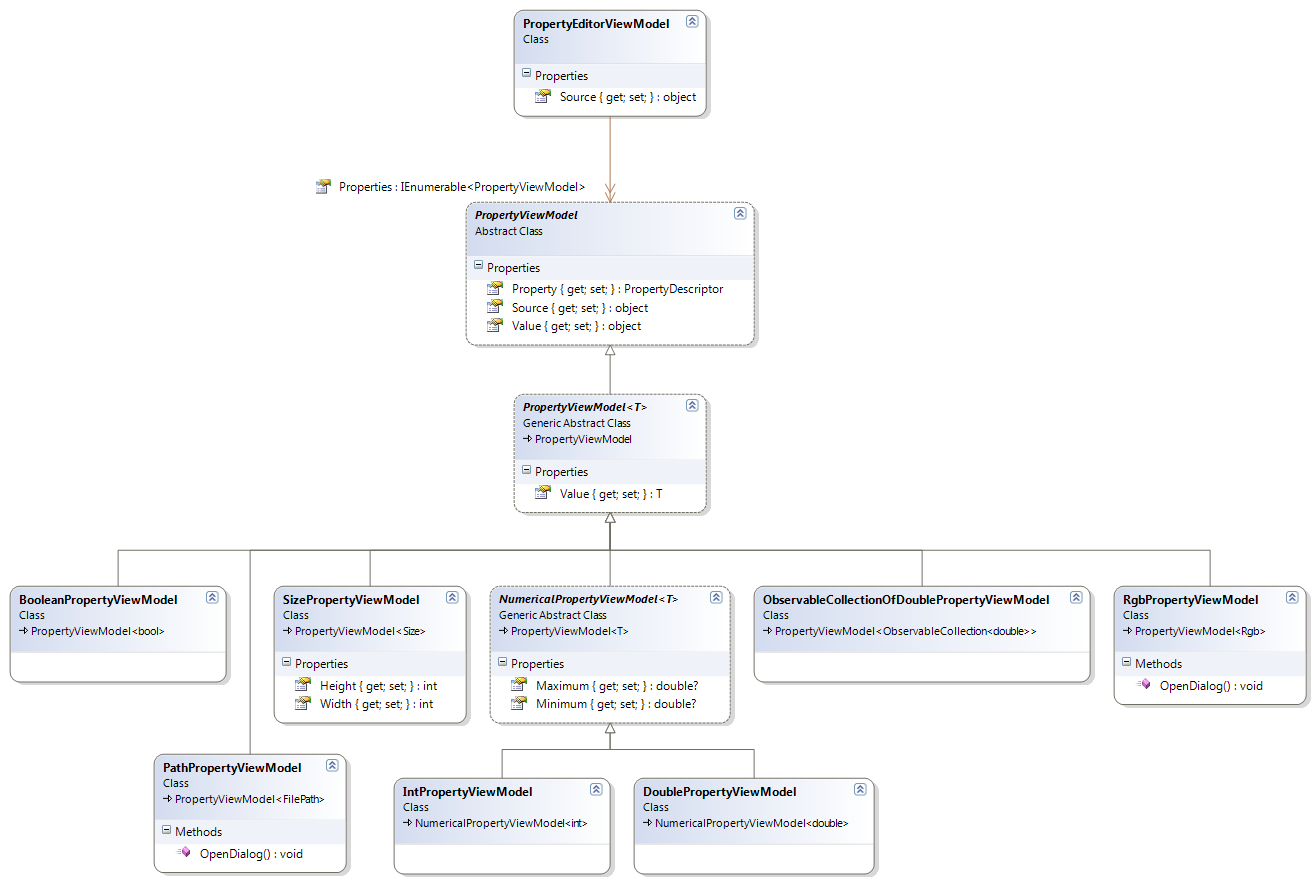
\includegraphics[width=\textwidth]{YuvKA.ViewModel.PropertyEditor/propertyEditor.png}
Diese Klassen dienen der Darstellung der vom Benutzer veränderbaren Properties mithilfe der View. 



\subsubsection{YuvKA.ViewModel.PropertyEditor.PropertyEditorViewModel}

\begin{verbatim}
public class PropertyEditorViewModel
\end{verbatim}

\paragraph{Beschreibung}~\\
Die Klasse \name{PropertyEditorViewModel} verwaltet eine Anzahl von Properties und ermöglicht ihre Darstellung mithilfe der View.

\paragraph{Typmember}
\begin{itemize}

\property{Properties}
	\begin{verbatim}
	public IEnumerable<PropertyViewModel> Properties { get; set; }
	\end{verbatim}
	Ruft die Liste der zu verwaltenden Properties ab oder legt sie fest.

\property{Source}
	\begin{verbatim}
	public object Source { get; set; }
	\end{verbatim}
	Ruft die Quelle der zu verwaltenden Properties ab oder legt sie fest.

\end{itemize}




\subsubsection{YuvKA.ViewModel.PropertyEditor.PropertyViewModel}

\begin{verbatim}
public abstract class PropertyViewModel
\end{verbatim}

\paragraph{Beschreibung}~\\
Abstrakte Oberklasse zu den einzelnen Property View Model Klassen.

\paragraph{Typmember}
\begin{itemize}
 	
\property{Property}
	\begin{verbatim}
	public PropertyDescriptor Property { get; set; }
	\end{verbatim}
	Ruft die Beschreibung der verwalteten Property ab oder legt sie fest.

\property{Source}
	\begin{verbatim}
	public object Source { get; set; }
	\end{verbatim}
	Ruft die Quelle der verwalteten Property ab oder legt sie fest.

\property{Value}
	\begin{verbatim}
	public object Value { get; set; }
	\end{verbatim}
	Ruft den Wert der verwalteten Property ab oder legt ihn fest.

\end{itemize}




\subsubsection{YuvKA.ViewModel.PropertyEditor.PropertyViewModel\textless T\textgreater}

\begin{verbatim}
public generic abstract class PropertyViewModel<T>
\end{verbatim}

\paragraph{Beschreibung}~\\
Abstrakte Klasse zur Darstellung der benötigten Properties mithilfe der View.

\paragraph{Typmember}
\begin{itemize}

\property{Value}
	\begin{verbatim}
	public T Value { get; set; }
	\end{verbatim}
	Ruft den Wert der Property ab oder legt ihn fest. T ist hierbei der Typ, der verwalteten Property.
\end{itemize}




\subsubsection{YuvKA.ViewModel.PropertyEditor.BooleanPropertyViewModel}

\begin{verbatim}
public class BooleanPropertyViewModel
\end{verbatim}

\paragraph{Beschreibung}~\\
Klasse zur Darstellung einer Property vom Typ \name{boolean} mithilfe der View. Hier ist lediglich der Typ der zu verwaltenden Property als \name{boolean} gesetzt.




\subsubsection{YuvKA.ViewModel.PropertyEditor.PathPropertyViewModel}

\begin{verbatim}
public class PathPropertyViewModel
\end{verbatim}

\paragraph{Beschreibung}~\\
Klasse zur Darstellung einer Property, welche einen Dateipfad darstellt.

\paragraph{Typmember}
\begin{itemize}

\method{OpenDialog}
	\begin{verbatim}
	public void OpenDialog()
	\end{verbatim}
	Öffnet einen Dialog zur Auswahl des Dateipfades.

\end{itemize}




\subsubsection{YuvKA.ViewModel.PropertyEditor.SizePropertyViewModel}

\begin{verbatim}
public class SizePropertyViewModel
\end{verbatim}

\paragraph{Beschreibung}~\\
Klasse zur Darstellung einer Property vom Typ \name{Size} mithilfe der View.

\paragraph{Typmember}
\begin{itemize}
	
\property{Height}
	\begin{verbatim}
	public int Height { get; set; }
	\end{verbatim}
	Ruft den \name{Height}-Wert der verwalteten \name{Size} Property ab oder legt ihn fest.

\property{Width}
	\begin{verbatim}
	public int Width { get; set; }
	\end{verbatim}
	Ruft den \name{Width}-Wert der verwalteten \name{Size} Property ab oder legt ihn fest.

\end{itemize}




\subsubsection{YuvKA.ViewModel.PropertyEditor.NumericalPropertyViewModel\textless T\textgreater}

\begin{verbatim}
public generic abstract class NumericalPropertyViewModel<T>
\end{verbatim}

\paragraph{Beschreibung}~\\
Abstrakte Klasse zur Darstellung einer numerischen Property mithilfe der View.

\paragraph{Typmember}
\begin{itemize}

\property{Maximum}
	\begin{verbatim}
	public Nullable<double> Maximum
	\end{verbatim}
	Ruft die obere Grenze des Wertes der verwalteten Property ab oder legt ihn fest.

\property{Minimum}
	\begin{verbatim}
	public Nullable<double> Minimum
	\end{verbatim}
	Ruft die untere Grenze des Wertes der verwalteten Property ab oder legt ihn fest.

\end{itemize}




\subsubsection{YuvKA.ViewModel.PropertyEditor.IntPropertyViewModel}

\begin{verbatim}
public class IntPropertyViewModel
\end{verbatim}

\paragraph{Beschreibung}~\\
Klasse zur Darstellung eines \name{int}-Wertes mithilfe der View. Hier ist lediglich der Typ der zu verwaltenden Property als \name{int} gesetzt.




\subsubsection{YuvKA.ViewModel.PropertyEditor.DoublePropertyViewModel}

\begin{verbatim}
public class DoublePropertyViewModel
\end{verbatim}

\paragraph{Beschreibung}~\\
Klasse zur Darstellung  eines \name{double}-Wertes mithilfe der View. Hier ist lediglich der Typ der zu verwaltenden Property als \name{double} gesetzt.




\subsubsection{YuvKA.ViewModel.PropertyEditor.ObservableCollectionOfDoublePropertyViewModel}

\begin{verbatim}
public class ObservableCollectionOfDoublePropertyViewModel
\end{verbatim}

\paragraph{Beschreibung}~\\
Klasse zur Darstellung einer \name{ObservableCollection} von \name{double}-Werten mithilfe der View.



\subsubsection{YuvKA.ViewModel.PropertyEditor.RgbPropertyViewModel}

\begin{verbatim}
public class RgbPropertyViewModel
\end{verbatim}

\paragraph{Beschreibung}~\\
Klasse zur Darstellung einer \name{Rgb} Property mithilfe der View.

\paragraph{Typmember}
\begin{itemize}
	
\method{OpenDialog}
	\begin{verbatim}
	public void OpenDialog()
	\end{verbatim}
	Öffnet einen Dialog zur Auswahl des Farbkanals.

\end{itemize}


